\chapter[Proposta de viabilização]{PROPOSTA DE VIABILIZAÇÃO}

\section{Solução do Sistema Embarcado}

Para o sistema embarcado será desenvolvido um algoritmo para realizar o processamento de imagem, para identificação de faixa de pedestre. Para esse projeto utilizaremos a placa Raspberry Pi que possui todos os recursos necessários para o desenvolvimento dos requisitos e capaz de realizar um processamento de imagem com qualidade.

\begin{figure}[h]
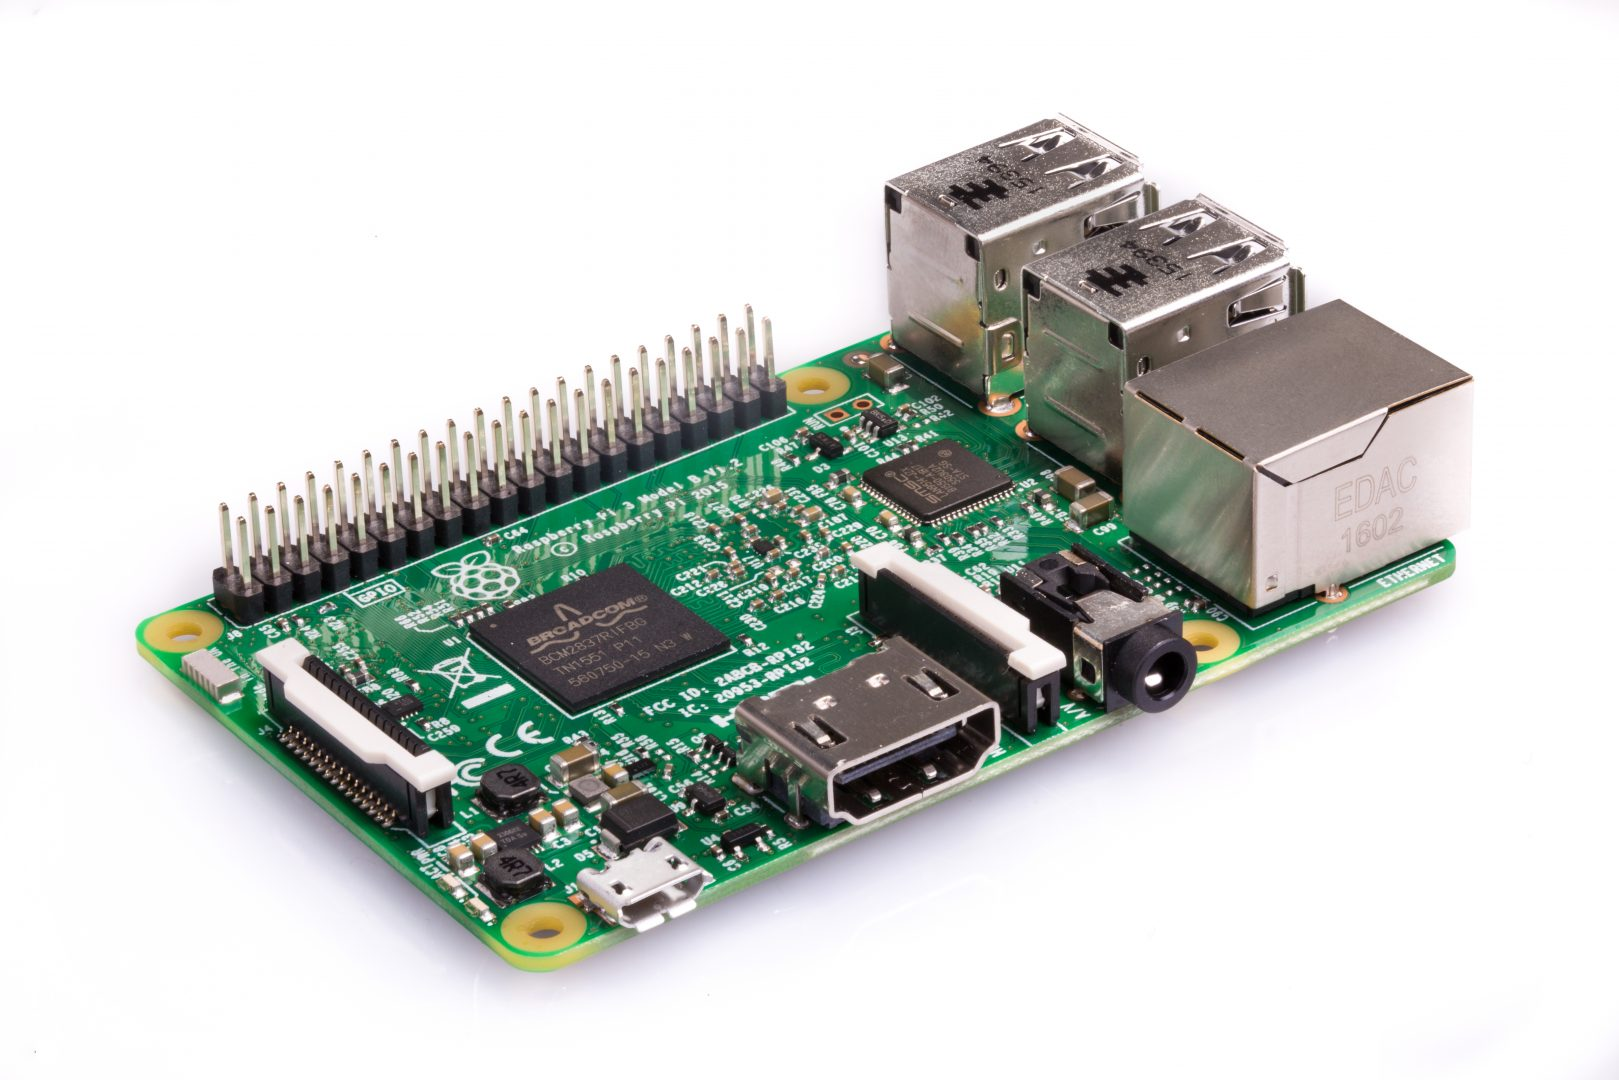
\includegraphics[scale=0.2]{figuras/Capitulo4/rasp.jpg}
\centering
\caption{Raspberry Pi.}
\label{fig:rasp.jpg}
Fonte: \cite{rasp}
\end{figure}

Para a realização do processamento de imagem usaremos a Pi.camera pelo seu tamanho compacto e de fácil utilização quando acoplado a raspberry.
\begin{figure}[h]
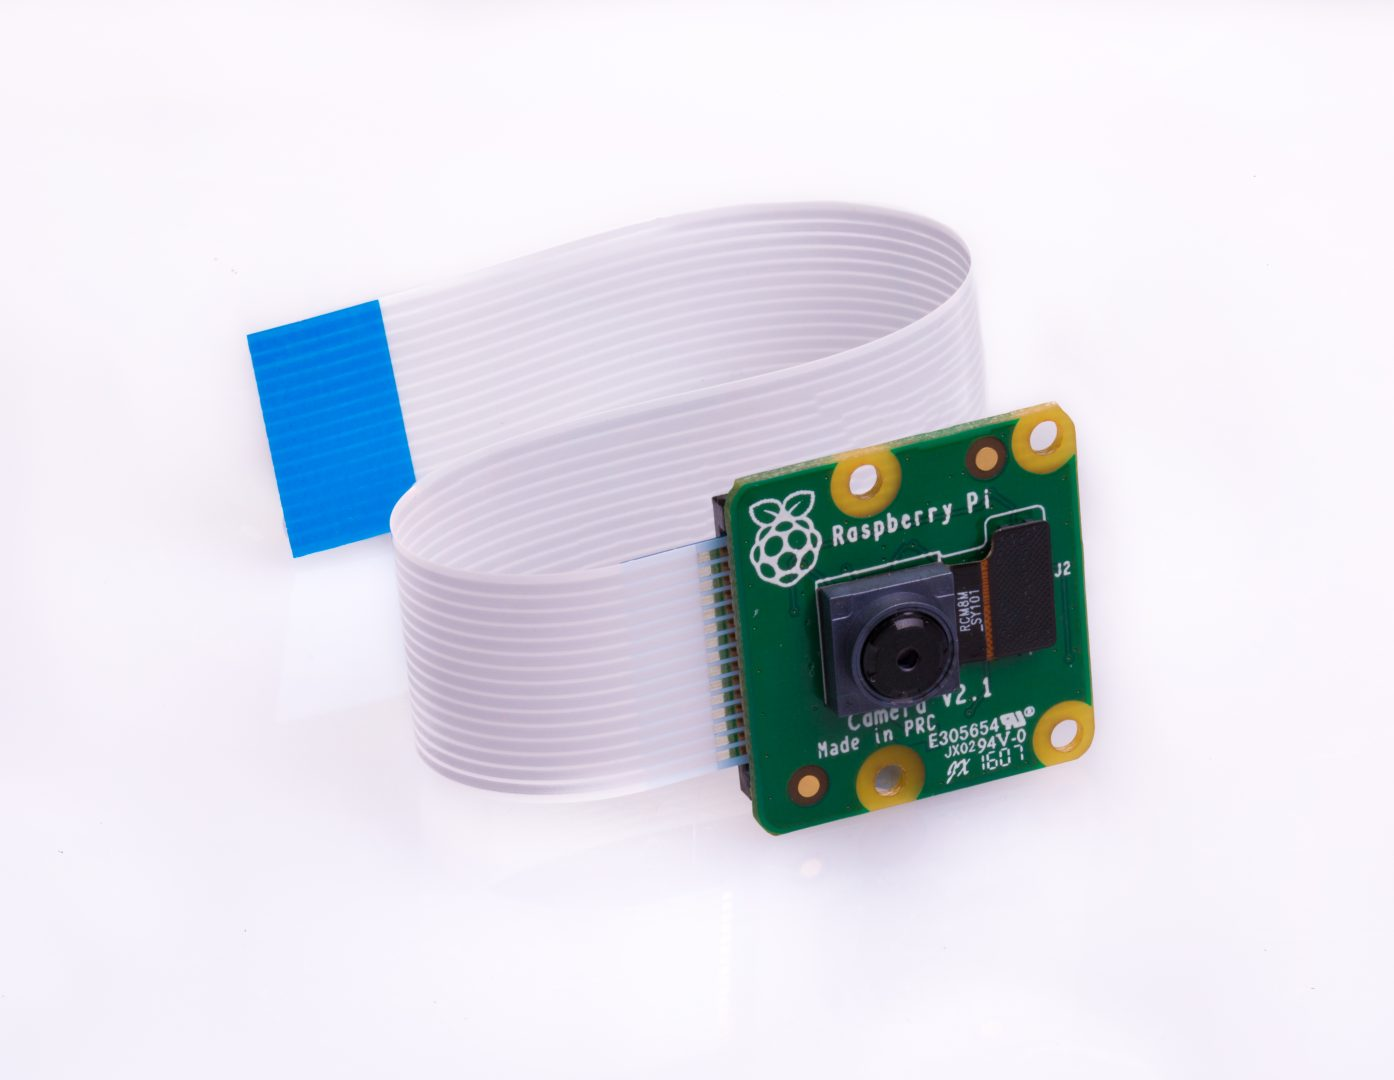
\includegraphics[scale=0.2]{figuras/Capitulo4/camera.jpg}
\centering
\caption{Pi câmera.}
\label{fig:camera.jpg}
Fonte: \cite{camera}
\end{figure}

Já para a realização do controle de todo o sensoriamento utilizaremos outro microcontrolador sendo ele responsável, pelo controle de todos os sensores ultrassônicos e de todos os vibracalls presente. Sendo de fundamental importância para a localização do deficiente visual. Desenvolveremos o algoritmo nesse recurso pelo seu tamanho reduzido facilitando assim a implementação na estrutura e devido ao seu consumo de corrente sendo bem menor aumentando assim a durabilidade da bateria.

\begin{figure}[h]
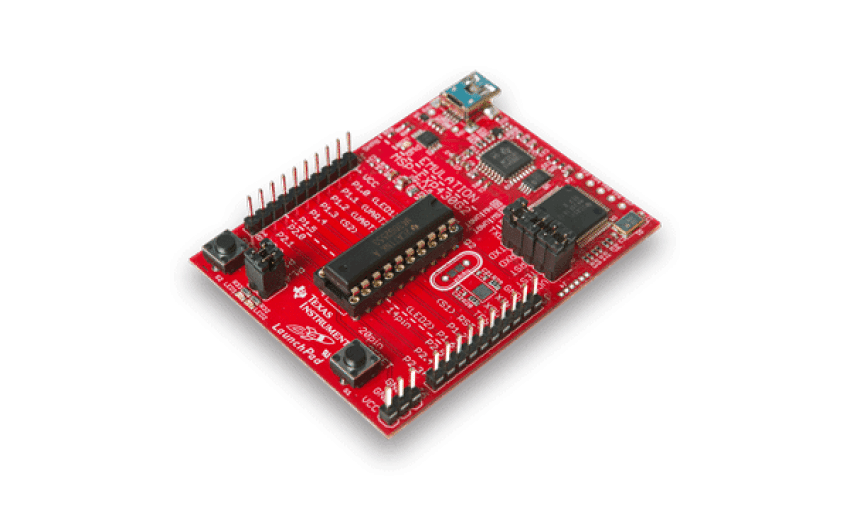
\includegraphics[scale=0.4]{figuras/Capitulo4/msp.png}
\centering
\caption{Microcontrolador MSP430.}
\label{fig:msp.png}
Fonte: \cite{msp}
\end{figure}

Na realização do sensoriamento serão utilizados sensores HC-SR04, sensores ultrassônicos, responsáveis por medir a proximidade do deficiente visual com obstáculos. Seu princípio de funcionamento está baseado na emissão de uma onda sonora de alta frequência, e na medição do tempo levado para a recepção do eco produzido quando esta onda se choca com o objeto.

\begin{figure}[h]
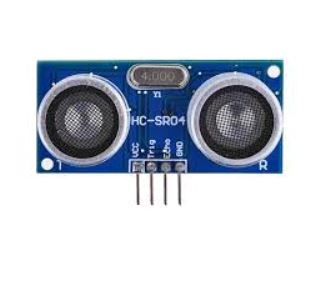
\includegraphics[scale=0.8]{figuras/Capitulo4/sensor.JPG}
\centering
\caption{Sensor Ultrassônico.}
\label{fig:sensor.jpg}
Fonte: \cite{sensor}
\end{figure}

